\documentclass[aps,prl,amsmath,amssymb,twocolumn,showpacs,showkeys,superscriptaddress]{revtex4-1}
%\documentclass[aip,apl,amsmath,amssymb,reprint,showpacs,showkeys,groupedaddress]{revtex4-1}
%\documentclass[aps,prl,amsmath,amssymb,preprint,showpacs,showkeys,superscriptaddress]{revtex4-1}

\usepackage{graphicx}% Include figure files
\usepackage{dcolumn}% Align table columns on decimal point
\usepackage{color}
\usepackage{ulem}
%\usepackage[showframe]{geometry}% http://ctan.org/pkg/geometry
%\usepackage{lipsum}% http://ctan.org/pkg/lipsum
%\usepackage{multicol}% http://ctan.org/pkg/multicols
\newcommand{\cl}[1]{\textcolor[rgb]{0.85,0,0}{#1}}
\newcommand{\ct}[1]{\textcolor[rgb]{0,0.7,0}{#1}}
\newcommand{\cf}[1]{\colorbox[rgb]{1,0.6,0.6}{\textcolor{black}{#1}}}
\newcommand{\cfs}[1]{\colorbox[rgb]{1,0.6,0.6}{\textcolor{black}{\sout{#1}}}}
\hyphenation{InGaAs}
\hyphenation{GaAs}
\hyphenation{InAs}


\begin{document}
%\title{Effect of second order piezoelectricity on electric dipole in strain-tuned InGaAs/GaAs quantum dots}
\title{Effect of second order piezoelectricity on excitonic structure of strain-tuned InGaAs/GaAs quantum dots}


\author{Petr Klenovsk\'y}
\email[]{klenovsky@physics.muni.cz}
\affiliation{Department of Condensed Matter Physics, Faculty of Science, Masaryk University, Kotl\'a\v{r}sk\'a~267/2, 61137~Brno, Czech~Republic}
\affiliation{Central European Institute of Technology, Masaryk University, Kamenice 753/5, 62500~Brno, Czech~Republic}

\author{Petr Steindl}
\affiliation{Department of Condensed Matter Physics, Faculty of Science, Masaryk University, Kotl\'a\v{r}sk\'a~267/2, 61137~Brno, Czech~Republic}
\affiliation{Central European Institute of Technology, Masaryk University, Kamenice 753/5, 62500~Brno, Czech~Republic}

\author{Johannes Aberl}
\affiliation{Institute of Semiconductor and Solid State Physics, Johannes Kepler University Linz, Altenbergerstra{\ss}e 69, A-4040 Linz, Austria}

\author{Eugenio Zallo}
\affiliation{Institute for Integrative Nanosciences, IFW Dresden, Helmholtzstra{\ss}e 20, D-01069 Dresden, Germany}
\affiliation{Paul-Drude-Institut f{\"u}r Festk{\"o}rperelektronik, Hausvogteilplatz 5-7, 10117 Berlin, Germany}

\author{Thomas Fromherz}
\affiliation{Institute of Semiconductor and Solid State Physics, Johannes Kepler University Linz, Altenbergerstra{\ss}e 69, A-4040 Linz, Austria}

\author{Armando Rastelli}
\affiliation{Institute of Semiconductor and Solid State Physics, Johannes Kepler University Linz, Altenbergerstra{\ss}e 69, A-4040 Linz, Austria}

\author{Rinaldo Trotta}
\affiliation{Institute of Semiconductor and Solid State Physics, Johannes Kepler University Linz, Altenbergerstra{\ss}e 69, A-4040 Linz, Austria}

\date{\today}

\begin{abstract}

We study the effects of nonlinear piezoelectricity on the electron-hole electric dipole moment in strain-tuned InGaAs/GaAs quantum dots. We investigate the influence of prestress, dot dimensions and indium distribution as well as various elements of the expansion of electrical polarization in terms of applied elastic stress. We find the presence of a large built-in in-plane stress due to the lattice mismatch provided by, e.g., a quantum dot necessary for the dipole inversion to occur. Based on the comparison of the effects of first- and second-order piezoelectricity we provide a simple relation to estimate the influence of applied stress on the electrical polarization in InGaAs quantum dots on GaAs substrates.

\end{abstract}

%\pacs{73.21.La, 75.75.-c, 85.35.Be, 68.65.Hb}
%
\pacs{78.67.Hc, 73.21.La, 85.35.Be, 77.65.Ly}

\maketitle

\section{Introduction}

Quantum dots (QDs), commonly referred as ``artificial atoms", are nanostructures that have zero-dimensional confinement and, thus, provide a number of appealing applications. Among others, QDs are sources of single photons for optical fibre communication~\cite{Huffaker1998}, secure optical links using entangled photon pairs~\cite{Trotta:16}, or quantum gates~\cite{Krapek2010,Klenovsky2016}. It is worth noting that also in the $\text{III-V}$ material system QDs might support spatially indirectly located electrons and holes~\cite{Klenovsky2015,Klenovsky2017} similar to the situation in SiGe QDs in a Si matrix \cite{2009NJoP_Brehm,KlenovskyPRB2012}. 

The importance of higher orders of the expansion of electrical polarization ${\bf P}$ as a function of strain $\eta$ was first highlighted by Bester and colleagues~\citep{Bester:06, Bester:06_2}. They have found that these terms might even dominate compared to the first order ones in $\mathrm{III-V}$ semiconductors particularly when $\eta$ is large, which is, e.g., the common property of self-assembled QDs obtained with the Stranski-Krastanow growth method~\cite{Grundmann:95}.

In Ref.~\cite{Aberl:17} we have recently shown that the vertical electron-hole dipole moment $p$ in InGaAs/GaAs QDs can be tuned by externally-applied, anisotropic in-plane stress~\cite{Trotta:12,Trotta:13} and even its inversion can be achieved. Furthermore, it was found that the pronounced tuning of $p$ can only be described by nonlinear terms in the expansion of the piezoelectric tensor. In this work we provide more details on the effects of the second-order piezoelectric terms on the tunability of $p$ leading us finally to an approximate relation between
${\bf P}$
%$p$ 
and the externally applied stress $\sigma^{(app)}$ applicable to the studies of strain-tunable InGaAs QDs. 

\section{Theory}

The Taylor expansion of ${\bf P}$ in terms of $\eta$ is obtained as
%
\begin{equation}
\label{eq:2ndPiezGeneral}
P_{\mu}=\sum_je_{\mu j}\eta_j+\frac{1}{2}\sum_{jk}B_{\mu jk}\eta_j\eta_k+\dots,
\end{equation}
%
where $e_{\mu j}$ is the linear and $B_{\mu jk}$ are the quadratic piezoelectric coefficients. It is well known that in $\mathrm{III-V}$ zinc blende semiconductors most of $e$ and $B$ terms are equal to each other or vanishing and only one linear ($e_{14}$) and three nonlinear ($B_{114}$, $B_{124}$, $B_{156}$) terms remain independent in Eq.\ref{eq:2ndPiezGeneral} up to the second order ~\cite{Beya-Wakata2011}. It is then convenient to rewrite Eq.~(\ref{eq:2ndPiezGeneral}) as ${\bf P}={\bf P}_{l}+{\bf P}_{nl}$, where ${\bf P}_{l}$ is the linear term
%
%
\begin{equation}
\label{eq:1stPiez}
{\bf P}_{l}=e_{14}\begin{pmatrix}\eta_4\\\eta_5\\\eta_6\end{pmatrix},
\end{equation}
%
and ${\bf P}_{nl}$ the nonlinear one:
%
\begin{equation}
\label{eq:2ndPiez}
{\bf P}_{nl}=B_{114}\begin{pmatrix}\eta_1\eta_4\\\eta_2\eta_5\\\eta_3\eta_6\end{pmatrix}+
B_{124}\begin{pmatrix}\eta_4(\eta_2+\eta_3)\\\eta_5(\eta_3+\eta_1)\\\eta_6(\eta_1+\eta_2)\end{pmatrix}+
B_{156}\begin{pmatrix}\eta_5\eta_6\\\eta_4\eta_6\\\eta_4\eta_5\end{pmatrix}.
\end{equation}
%
%
Here $\eta$-s are indexed according to the Voigt notation,~i.e.,~ $\eta_1=\eta_{xx}$, $\eta_2=\eta_{yy}$, $\eta_3=\eta_{zz}$, $\eta_4=2\eta_{yz}$, $\eta_5=2\eta_{xz}$, $\eta_6=2\eta_{xy}$~\cite{Beya-Wakata2011} where $x,y,z$ denote the crystallographic axes of the conventional cubic unit cell of the zinc blende lattice.
%
%$1=xx,2=yy,3=zz,4=yz,5=xz,6=xy$~\cite{Beya-Wakata2011}.
%
Note that even though the coefficients of the expansion into cubic
%higher order 
terms was provided by Tse and colleagues~\cite{Tse2013}, we restrict ourselves to second-order ones in this work and show that for the small externally applied strain magnitude of only 0.1~\%~\cite{Aberl:17} we can describe our experimental results accurately within this restriction. 


\section{Results}

\begin{figure}[!ht]
\renewcommand{\tabcolsep}{2pt}
\begin{center}
\begin{tabular}{c}
%\includegraphics[width=0.45\textwidth]{QDstruct.eps} \\
%\includegraphics[width=0.45\textwidth]{structura_wo-gradient.eps} \\
%\includegraphics[width=0.42\textwidth]{structura_wo-gradient_w_triangles.eps}
%\includegraphics[width=0.42\textwidth]{171206_structura_wo-gradient_w_triangles_and_wfuncions_vs2.eps} \\
%\includegraphics[width=0.42\textwidth]{171206_structura_wo-gradient_w_triangles_and_wfuncions_vs3_oprava.eps} \\
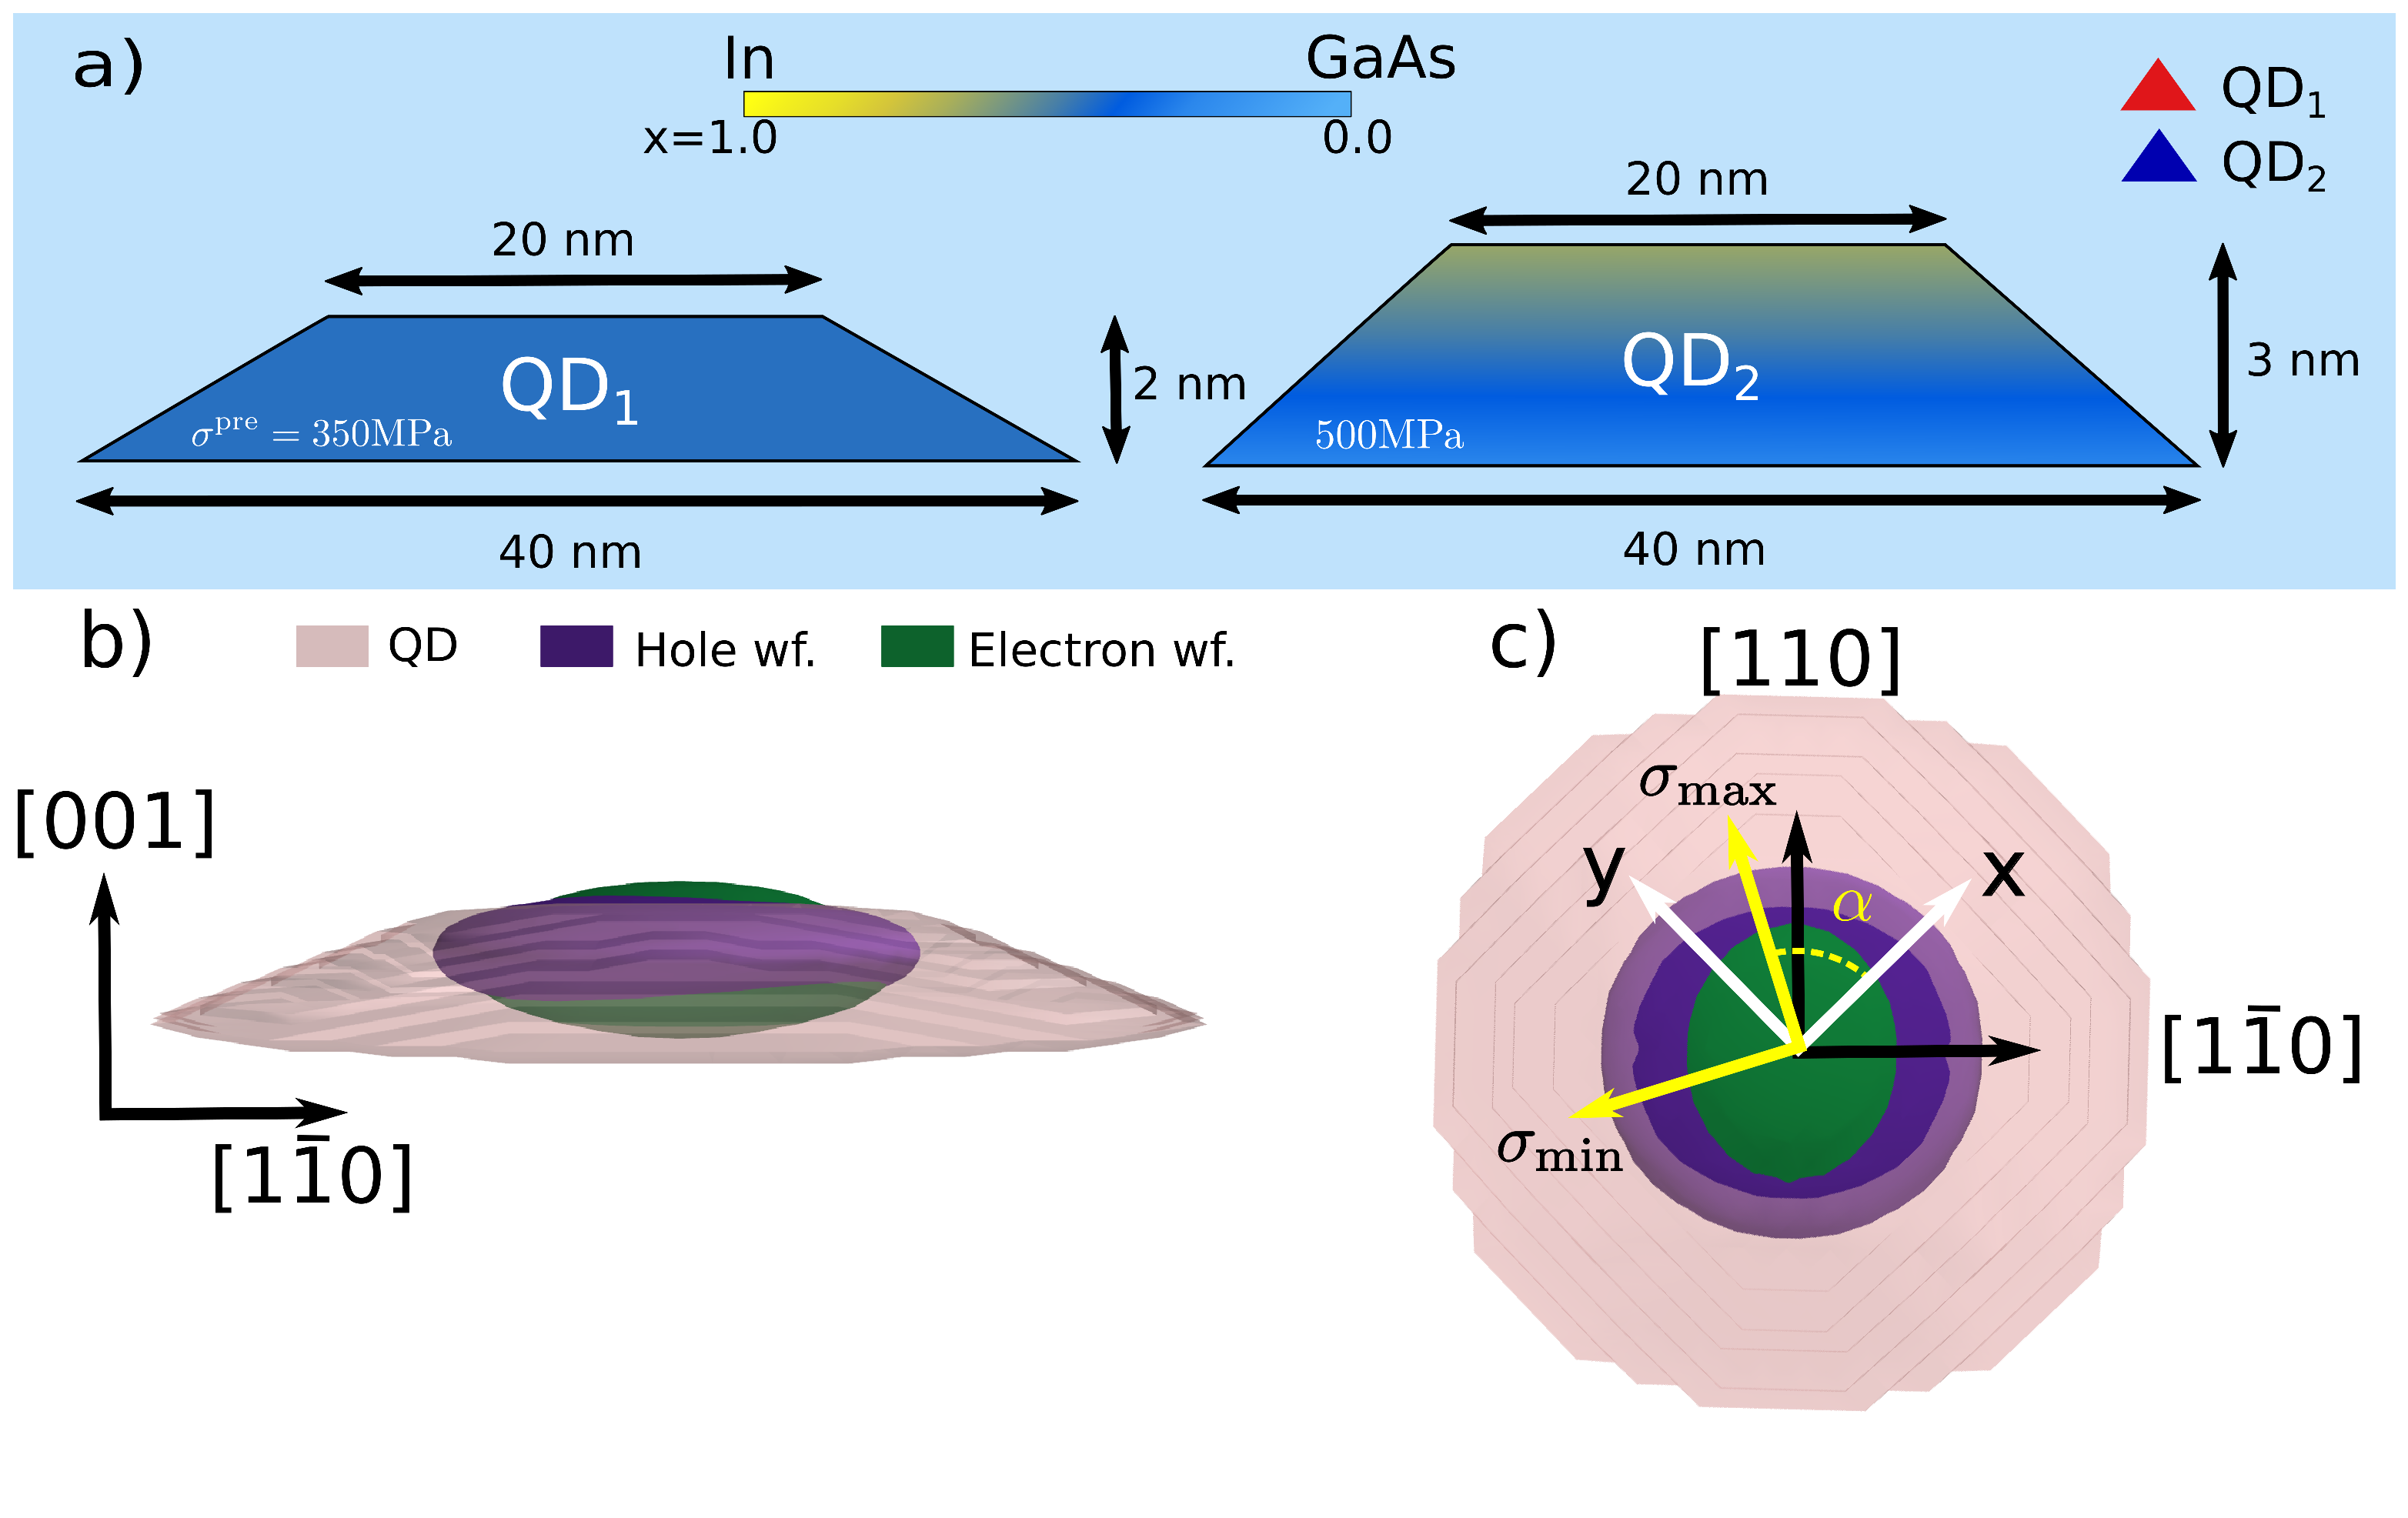
\includegraphics[width=0.42\textwidth]{180204_structura_wo-gradient_w_triangles_and_wfuncions_vs5.eps} \\ 
\end{tabular}
\end{center}
\caption{In panel a) we show the side view of the calculated In$_{{x}}$Ga$_{1-x}$As/GaAs QD$_1$ and QD$_2$ structures. The shape of both QDs is that of truncated cones. The base and top diameters of QD$_1$~(QD$_2$) are 40~nm~(40~nm) and 20~nm~(20~nm), respectively, the height is 2~nm~(3~nm), and In composition is linearly increasing from 0.45~(0.25) at the bottom to 0.45~(0.65) at the apex. Panels b) and c) show the top and side view, respectively, of the typical simulated dot (grey), and calculated electron (green) and hole (blue) probability densities. The wavefunctions are
given as isosurfaces encircling 70\% of the probability.
\label{fig:QDStruct}}
\end{figure}


Before we present the results of full electronic structure calculations for the InGaAs QDs obtained by the nextnano$^3$ simulation suite~\cite{Birner:07}, we analyze the additional piezoelectric polarization established by the externally applied stress. In particular, we show that despite the small strains established in the InGaAs layer as a consequence of deformation of a piezo actuator the sample is bonded on, the established piezo-polarisation is dominated by the second order piezo-constants $B_{\mu,j,k}$. For simplicity, in this section we tread the InGaAs QD as two-dimensional layer with tetragonal symmetry.    



For comparison, We have calculated the electronic structure of InGaAs/GaAs QDs with the shape of truncated cones as shown in Fig. \ref{fig:QDStruct} aI using the envelope function approximation based on 8-band ${\bf k}\cdot{\bf p}$ perturbation method using the nextnano$^3$ simulation suite~\cite{Birner:07}. The calculations include full treatment of the elastic strain field employing the Bir-Pikus hamiltonian~\cite{Bir:74}. Piezoelectric fields up to the second order in the strain are included selfconsistently.  We have simulated two structures that we call QD$_1$ and QD$_2$ differing in size and In alloy distribution.
Side views of QD$_1$ and QD$_2$ are shown in Fig.~\ref{fig:QDStruct}~a) and their parameters were deliberately chosen so that the calculated dependencies of the emission energy $E_0$ and of the dipole moment $p$ on the hydrostatic part of the applied anisotropic stress $\sigma_{\mathrm{max}}+\sigma_{\mathrm{min}}$ match the experimental results taken from Ref.~\cite{Aberl:17}, see Fig.~\ref{fig:TheorVsExp}. The variables $\sigma_{\mathrm{max}}$ and $\sigma_{\mathrm{min}}$ denote the principal stresses~\cite{Trotta:15} applied externally by the two-dimensional piezo actuator. In  Ref.~\citep{Aberl:17} it was shown that $\sigma_{\mathrm{max}}$ was applied at an angle of $\alpha=55^{\circ}$ with respect to the crystal axis [100], resulting in the principal axis system of the externally applied stress as shown in   Fig. \ref{fig:QDStruct}. The various coordinate systems used in our model as well as the single-particle wavefunctions of electrons and holes are indicated in Fig. \ref{fig:QDStruct} b) and c).
%
%
%
\begin{figure}[!ht]
\renewcommand{\tabcolsep}{2pt}
\begin{center}
\begin{tabular}{c}
%\includegraphics[width=0.42\textwidth]{2017-12-15__170921_35deg_pres200___theoryVSexperiment.eps} \\
\includegraphics[width=0.42\textwidth]{2018-02-04__171219_8x8_neotocena_++_nn+_35deg_pres500___theoryVSexperiment.eps} \\
\end{tabular}
\end{center}
\caption{
Dependencies of $E_0$ (top panel) and $p/e$ (bottom panel) on $\sigma_{\mathrm{max}}+\sigma_{\mathrm{min}}$ experimentally obtained from $\mu$PL measurements of nine InGaAs QDs~\cite{Aberl:17} (broken curves) and that calculated for QD$_1$ (full red curve) and QD$_2$ (full blue curve). The letter $e$ denotes the elementary charge.
%
%two different QDs, i.e. first with base and top diameter of 30~nm and 15~nm, respectively and height of 3~nm. 
\label{fig:TheorVsExp}}
\end{figure}


As discussed in Ref. \cite{Aberl:17}, in course of bonding the sample onto the piezo actuator, a pre-stess $\hat\sigma^\text{Pre}$ independent on the voltage applied to the piezo is exerted on the sample. Remarkably, excellent agreement with experiment is obtained for $\sigma^{\mathrm{pre}}=200$~MPa by only slightly changing the properties of simulated QDs well within realistic limits as seen in Fig.~\ref{fig:TheorVsExp}. This suggests a rather general applicability of our method for modeling of the stress-tuned InGaAs/GaAs QD structures.

\begin{figure}[!ht]
\renewcommand{\tabcolsep}{2pt}
\begin{center}
\begin{tabular}{c}
%\includegraphics[width=0.4\textwidth]{45deg/2017-10-04__170921_45deg_pres200.00___theoryVSexperiment.eps} \\
%\includegraphics[width=0.4\textwidth]{171006_35deg_prestress/2017-10-06__170921_35deg_pres500.00___prestress.eps} \\
%
%\includegraphics[width=0.4\textwidth]{2017-12-15__170921_35deg_pres500___prestress.eps} \\ 
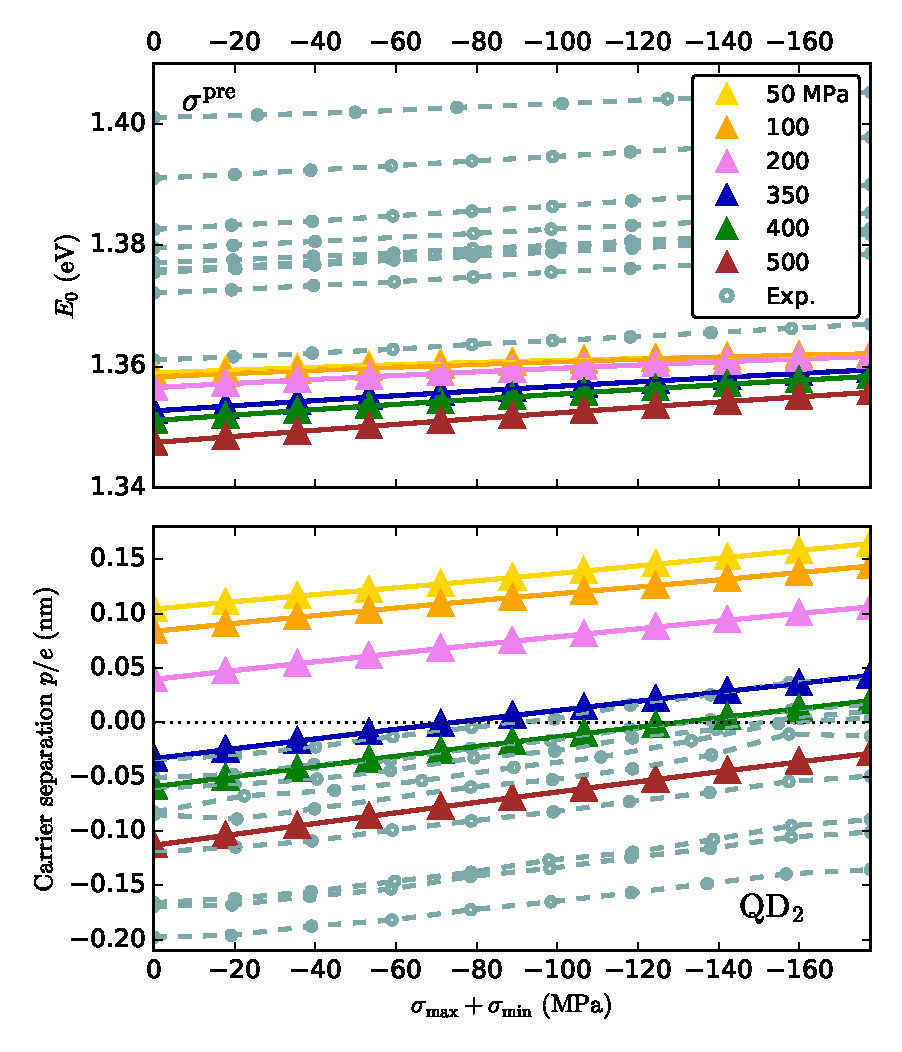
\includegraphics[width=0.4\textwidth]{FINAL__171219_8x8_neotocena_++_nn+_35deg_pres500___prestress.eps} \\
\end{tabular}
\end{center}
\caption{
Dependencies of $E_0$ (top panel) and $p/e$ (bottom panel) on $\sigma_{\mathrm{max}}+\sigma_{\mathrm{min}}$ experimentally obtained from $\mu$PL measurements of nine InGaAs QDs~\cite{Aberl:17} (broken curves) and that calculated for different values of $\sigma^{\mathrm{pre}}$. Except of $\sigma^{\mathrm{pre}}$ the simulated QDs had the same properties as QD$_2$. The letter $e$ denotes the elementary charge.
\label{fig:TuningByPrestress}}
\end{figure}
%
%
\begin{figure}[!ht]
\renewcommand{\tabcolsep}{2pt}
\begin{center}
\begin{tabular}{c}
%\includegraphics[width=0.4\textwidth]{45deg/2017-10-04__170921_45deg_pres200.00___theoryVSexperiment.eps} \\
%\includegraphics[width=0.4\textwidth]{2017-12-08__170921_35deg_pres200d00___30x15_height.eps} \\
\includegraphics[width=0.4\textwidth]{2018-02-05__171219_8x8_neotocena_++_nn+_35deg_pres350___40x20_height.eps} \\
\end{tabular}
\end{center}
\caption{
Dependencies of $E_0$ (top panel) and $p/e$ (bottom panel) on $\sigma_{\mathrm{max}}+\sigma_{\mathrm{min}}$ experimentally obtained from $\mu$PL measurements of nine InGaAs QDs~\cite{Aberl:17} (broken curves) and that calculated for different values of dot height. Except of height the simulated QDs had the same properties as QD$_2$ including the value of $\sigma^{\mathrm{pre}}=200$~MPa. The letter $e$ denotes the elementary charge.
\label{fig:TuningByHeight}}
\end{figure}
%

However, similar results can be obtained for different values of $\sigma^{\mathrm{pre}}$ acting on QD$_2$, see Fig.~\ref{fig:TuningByPrestress}, or different dot heights, see Fig.~\ref{fig:TuningByHeight}. Interestingly while $\sigma^{\mathrm{pre}}$ considerably influences the overall magnitude of $p$ it only mildly affects the slope $\partial p/\partial(\sigma_{\mathrm{max}}+\sigma_{\mathrm{min}})$ or the values of $E_0$. On the other hand, dot height influences all three parameters, i.e. $p$, $\partial p/\partial(\sigma_{\mathrm{max}}+\sigma_{\mathrm{min}})$, and $E_0$ substantially.


\begin{figure}[!ht]
\renewcommand{\tabcolsep}{2pt}
\begin{center}
\begin{tabular}{c}
%\includegraphics[width=0.4\textwidth]{2017-12-15__170921_35deg_pres200___30x15x3_concentration.eps} \\
\includegraphics[width=0.4\textwidth]{2018-02-06__171219_8x8_neotocena_++_nn+_35deg_pres350___40x20x3_concentration} \\
\end{tabular}
\end{center}
\caption{
Dependencies of $E_0$ (top panel) and $p/e$ (bottom panel) on $\bigwedge_{\mathrm{max}}+\sigma_{\mathrm{min}}$ experimentally obtained from $\mu$PL measurements of nine InGaAs QDs~\cite{Aberl:17} (broken curves) and that calculated for different In contents inside QD. The data for In content linearly varying as a function of vertical dimension from 0.25~(0.65) at QD base to 0.65~(0.25) at QD apex are shown as blue~(orange) curves. Those for constant In content of 0.45 are given as green curves. The data calculated assuming second-(first-)order piezoelectricity taken from Ref.~\citep{Beya-Wakata2011} are given as full(open) triangles. All other properties of the dots we the same as for QD$_2$. The letter $e$ denotes the elementary charge.
\label{fig:TuningByConc}}
\end{figure}
%

Motivated by Refs.~\cite{Fry:00,Grundmann:95} discussing the influence of indium distribution inside InAs/GaAs QDs on $p$ we have also studied the effect of that in our stress-tuned dots. In Fig.~\ref{fig:TuningByConc} we show $E_0$ and $p$ as a function of $\sigma_{\mathrm{max}}+\sigma_{\mathrm{min}}$ for In contents (i) linearly increasing from 0.25 at the QD base to 0.65 at it apex, (ii) the same but for reverted concentration profile and (iii) for constant In composition of 0.45. Clearly, we find that $p/e$ where $e$ is the elementary charge at $\sigma_{\mathrm{max}}+\sigma_{\mathrm{min}}=0$ can be varied considerably by changing the slope of In content from $-0.05$~nm for (i) to $-0.27$~nm for (ii). The case (iii) is found in between at $-0.21$~nm. Note that previous values were obtained assuming second-order piezoelectricity. The data calculated with only first-order piezoelectricity show similar trends in agreement with the results of Refs.~\cite{Fry:00,Grundmann:95}. Noticeably, both $E_0$ and $\partial E_0/\partial(\sigma_{\mathrm{max}}+\sigma_{\mathrm{min}})$ do not depend appreciably on In distribution and only the mean value of In concentration is important.

However, the slopes $1/e\times\partial p/\partial(\sigma_{\mathrm{max}}+\sigma_{\mathrm{min}})$ differ considerably in case of first- and second-order piezoelectricity. We find the values of the fitted slopes in the former case in the range from 0.074 to 0.1~nm/GPa while for the latter they are between 0.42 and 0.55~nm/GPa. Slopes of the experimental data are between 0.42 and 0.5~nm/GPa. The relative error of all fitted slopes is $\approx$5\%, see also Sec.~SI in the supplementary material for the list of all fitted values and their errors. Thus, very good agreement is found between calculations assuming second-order piezoelectricity and experiment rather than for the first-order, see also Ref.~\cite{Aberl:17}. We will return to this point in the following.


%\onecolumngrid


\begin{figure}[!ht]
\renewcommand{\tabcolsep}{2pt}
\begin{center}
\begin{tabular}{c}
%\includegraphics[width=0.42\textwidth]{2017-12-15__170921_35deg_pres200___30x15x3_piezo2ndorder.eps} \\
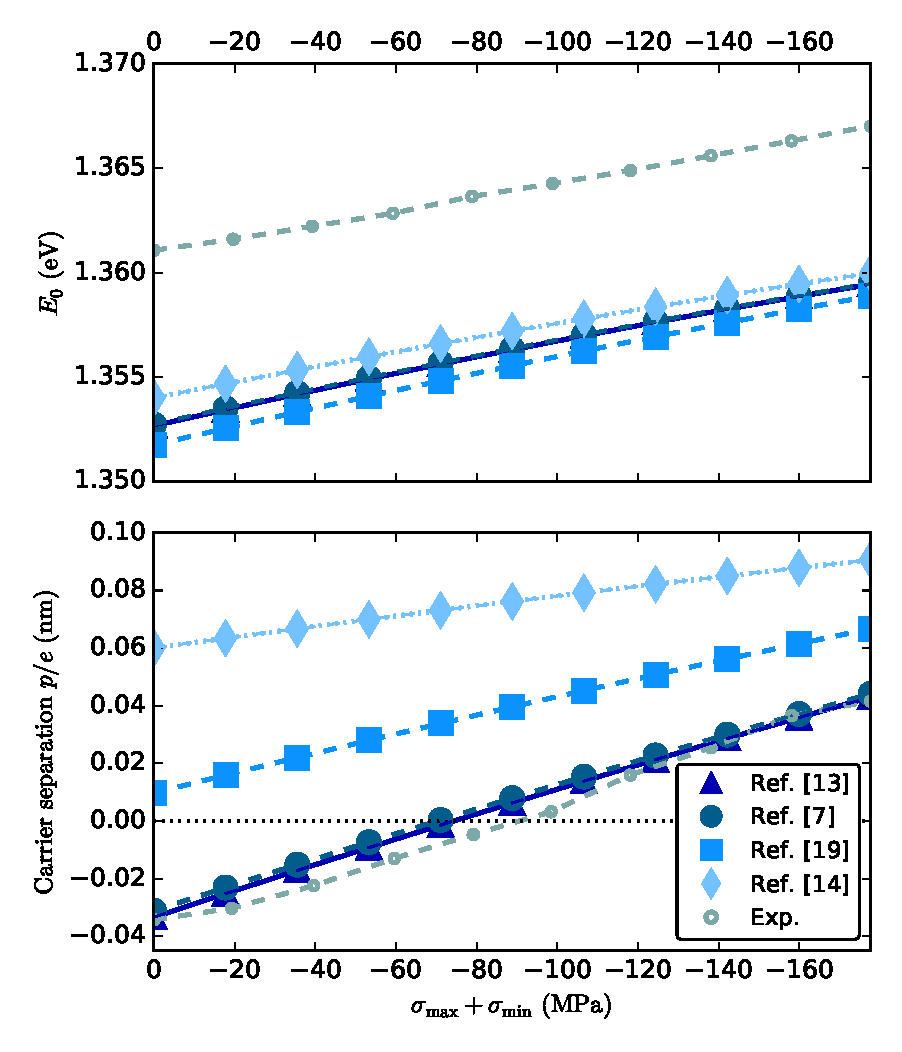
\includegraphics[width=0.42\textwidth]{2018-02-04__171219_8x8_neotocena_++_nn+_35deg_pres350___40x20x3-25-65_350_piezo2ndorder.eps} \\
\end{tabular}
\end{center}
\caption{
Comparison of calculation results based on four published sets of parameters of second order piezoelectric coefficients, i.e., Refs.\cite{Beya-Wakata2011,Bester:06,Caro:15,Tse2013} for QD$_2$. We show in the top panel the dependence of emission energy $E_0$ on applied stress $\sigma_{\mathrm{max}}+\sigma_{\mathrm{min}}$ and that for $p/e$ in lower panel. The experimental data from Ref.~\cite{Aberl:17} are shown by the grey broken curves in both panels. 
\label{fig:DiffPiezo}}
\end{figure}


We now proceed with the analysis of the evolution of $p/e$ on $\sigma_{\mathrm{max}}+\sigma_{\mathrm{min}}$ for all published second-order piezoelectric parameters, see also the supplementary material of Ref.~\cite{Aberl:17}. 
The results for QD$_2$ are shown in Fig.~\ref{fig:DiffPiezo} and demonstrate that both the inversion of $p$ with $\sigma_{\mathrm{max}}+\sigma_{\mathrm{min}}$ as well as the slopes $\partial p/\partial(\sigma_{\mathrm{max}}+\sigma_{\mathrm{min}})$ and $\partial E_0/\partial(\sigma_{\mathrm{max}}+\sigma_{\mathrm{min}})$ remain remarkably similar among various parameter sets in the literature even though the coefficients differ considerably among them.
For example, the parameter $B_{156}$ has even a different sign between Refs.~\cite{Bester:06} and~\cite{Beya-Wakata2011} or is omitted in Ref.~\cite{Tse2013}. For similar results of QD$_1$ see Fig.~S1 in the supplementary material.



\begin{figure}[!ht]
\begin{center}
%\includegraphics[width=0.42\textwidth]{2017-12-15__170921_35deg_pres200___30x15x3_piezo2ndorder_jednotlive_cleny.eps}
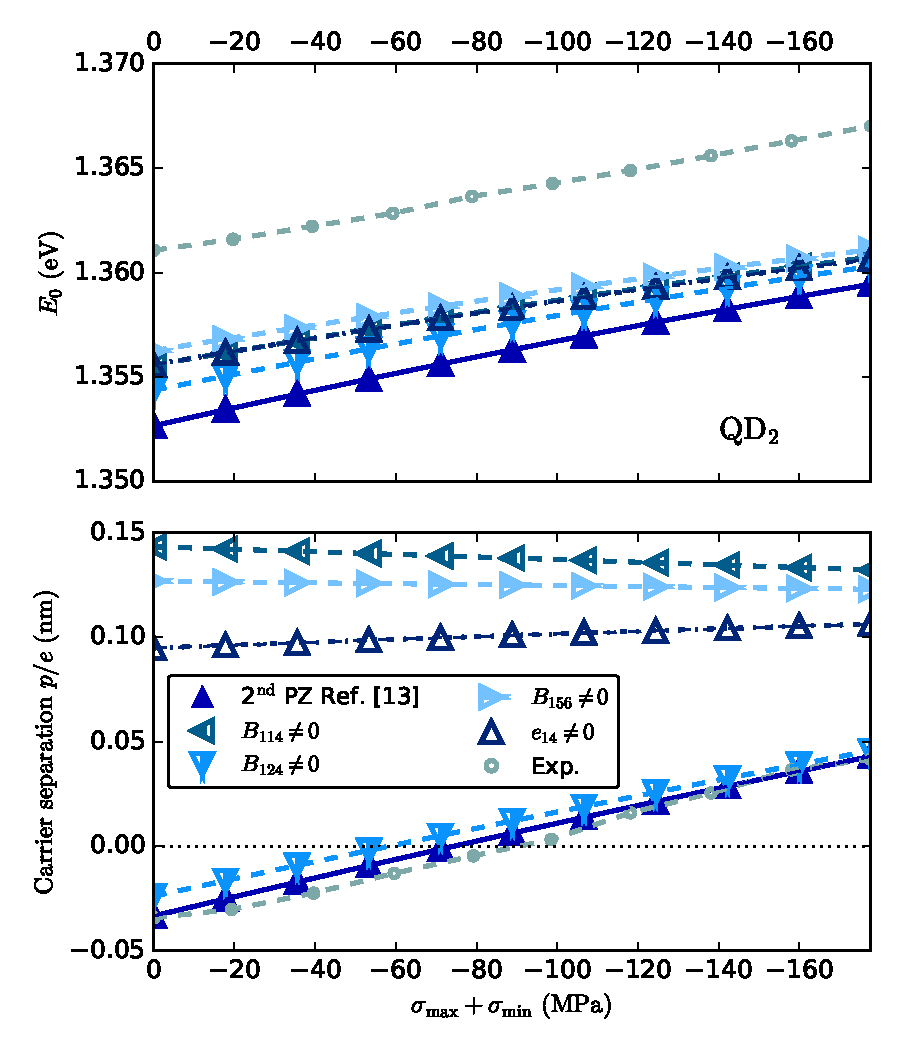
\includegraphics[width=0.42\textwidth]{2018-02-05__171219_8x8_neotocena_++_nn+_35deg_pres350___40x20x3_piezo2ndorder_jednotlive_cleny.eps}
\end{center}
\caption{
Comparison of dependencies of $E_0$ and $p/e$ on $\sigma_{\mathrm{max}}+\sigma_{\mathrm{min}}$ for all piezoelectric parameters equal to zero except of $e_{14}$, $B_{114}$, $B_{124}$, and $B_{156}$ sequentially retaining their values for QD$_2$. For comparison, one set of the experimental data from Ref.~\cite{Aberl:17} is given by the grey broken curve. Otherwise the outline of the figure is the same as that in Fig.~\ref{fig:DiffPiezo}.
\label{fig:DiffPiezoCoeff}}
\end{figure}

To investigate the origin of that apparent similarity we have performed calculations, in which we have set all piezoelectric parameters equal to zero except of $e_{14}$, $B_{114}$, $B_{124}$, and $B_{156}$ sequentially retaining their values, see Fig.~\ref{fig:DiffPiezoCoeff} for results for QD$_2$ and Fig.~S2 in the supplement for QD$_1$. 


Firstly, we note again that the dependencies for $E_0$ are very similar irrespective of which piezoelectric parameter is not set to zero. This is connected with the fact that the change of the emission energy from QDs with stress is dominated by its hydrostatic components.

Secondly, the most important piezoelectric parameter is noticeably $B_{124}$. Evidently, the second term in Eq.~(\ref{eq:2ndPiez}) dominates the dependencies of $E_0$ and $p/e$ on $\sigma_{\mathrm{max}}+\sigma_{\mathrm{min}}$. This is not surprising since the magnitude of $B_{124}$ is several times larger than that of $e_{14}$, $B_{114}$, or $B_{156}$~\cite{Beya-Wakata2011}. 
%
%Together with the effect on $E_0$ this underlines the importance of large hydrostatic in-plane built-in stress needed to be present in the system in order for the nonlinear piezoelectricity to be of importance. 

Since the possibilities of applying large stresses externally is presently limited, the presence of a large in-plane stress $\sigma^{\rm{in}}$ built-in the system is necessary for the observations of such large changes of $p$ and $E_0$ with applied stress. Together with the externally applied stress $\sigma^{\rm{app}}=\sigma_{\mathrm{max}}+\sigma_{\mathrm{min}}$ and taking into account also $\sigma^{\rm{pre}}$ we can describe the total anisotropic stress acting in the system as 
%
%
%
% %Note, that built-in stress 
%can be provided by, e.g., a nanostructure from lattice mismatched material like QD. 
%
%If we now decompose the built-in stress $\sigma^{\rm{in}}$ which is due to the lattice mismatch into its principal components $\sigma^{\rm{in}}_{\mathrm{max}}$ and $\sigma^{\rm{in}}_{\mathrm{min}}$ similarly as $\sigma_{\mathrm{max}}$ and $\sigma_{\mathrm{min}}$ for the externally applied stress $\sigma^{\rm{app}}$ and taking into account also the shear prestress $\sigma^{\rm{pre}}$ originating, e.g., from bonding of piezoelectric actuator to the sample we can describe the total anisotropic stress acting in the system as 
%
%
\begin{equation}
\label{eq:stressTot}
\sigma^{\rm{tot}} = \sigma^{\rm{tot}}_{\mathrm{max}}+\sigma^{\rm{tot}}_{\mathrm{min}} = \sigma^{\rm{in}} + \sigma^{\rm{pre}} + \sigma^{\rm{app}}.
\end{equation}
%
where $\sigma^{\rm{tot}}_{\mathrm{max}}$ and $\sigma^{\rm{tot}}_{\mathrm{min}}$ are total principal stresses.
%
%where $\sigma^{\rm{in}}=\sigma^{\rm{in}}_{\mathrm{max}}+\sigma^{\rm{in}}_{\mathrm{min}}$ and $\sigma^{\rm{app}}=\sigma_{\mathrm{max}}+\sigma_{\mathrm{min}}$ is the stress applied by the external actuator. 



%
Strikingly, the inspection of Fig.~\ref{fig:DiffPiezoCoeff} again reveals that linear piezoelectricity alone has only a small effect on $p$ and $E_0$. 
This suggests that instead of the commonly used
relation $|{\bf P}|=e_{14}\eta_{xy}$~\cite{YuCardona,Fry:00} for description of the effects of piezoelectricity, more realistic results might be obtained by
%
\begin{equation}
\label{eq:PiezApprox}
|{\bf P}|=2B_{124}\,\eta_{xy}(\eta_{xx}+\eta_{yy})=B_{124}\,(\eta^2_{\mathrm{max}}-\eta^2_{\mathrm{min}})\sin2\alpha
\end{equation}
%
%
%
%
where $\eta_{\mathrm{max}}$ and $\eta_{\mathrm{min}}$ are the principal strains, see also Sec.~SIII in the supplemental material for the derivation of Eq.~(\ref{eq:PiezApprox}). The strains $\eta_i$ are related to $\sigma^{\rm{tot}}_i$ in Eq.~(\ref{eq:stressTot}) by $\eta_i=2\sigma^{\rm{tot}}_i(1+\nu)/E$, where $\nu$ and $E$ are the Poisson ratio and the Young modulus, respectively, and $i\in{\{\mathrm{max}, \mathrm{min}\}}$. Even though Eq.~(\ref{eq:PiezApprox}) is not as general as Eqs.~(\ref{eq:1stPiez}) and~(\ref{eq:2ndPiez}) it provides a simple yet accurate approximation for the description of strain induced changes of ${\bf P}$ in nanostructures.
%



Finally, Fig.~\ref{fig:DiffPiezoCoeff} also shows the relative unimportance of the parameter $B_{156}$ and, therefore, confirms the feasibility of its omission as suggested in Ref.~\cite{Tse2013}.




\section{Conclusions}
We have studied the effects of nonlinear piezoelectricity on emission energy and electric dipole moment in InGaAs/GaAs quantum dots and pinpointed the importance of that for studies of those systems as compared to using first-order terms only. Also, we have elucidated the necessity of the presence of a large built-in in-plane stress due to the lattice mismatch in order for the pronounced changes of the electron-hole dipole due externally applied stress to occur. Furthermore, we have pinpointed the dominant piezoelectric term and provided an approximate relation to estimate the influence of the applied stress on electrical polarization in quantum dots.



\section{Acknowledgements}
P.K. would like to thank prof. Dieter Bimberg for fruitful discussions. A part of the work was carried out under the project CEITEC 2020 (LQ1601) with financial support from the Ministry of Education, Youth and Sports of the Czech Republic under the National Sustainability Programme II. The authors P.K., P.S., T.F., A.R., and R.T. were supported by the project MOBILITY of the Ministry of education, youth and sports of Czech republic under code 7AMB17AT044.

%The work was supported by the project no. TH01010419 of the Technological agency of the Czech republic, the European Regional Development Fund, project
%No. CZ.1.05/1.1.00/02.0068, and the European Social Fund, grant No. CZ.1.07/2.3.00/30.0005.

\bibliography{paper_jasz.bib}

\end{document}
